\documentclass[12pt]{article}
\usepackage[a4paper,margin=1in]{geometry}
\usepackage{setspace}
\usepackage{amsmath}
\usepackage{amssymb}
\usepackage{graphicx}
\usepackage{booktabs}
\usepackage{makecell}
\usepackage{graphicx}
\usepackage{tabularx}
\usepackage{float}
\usepackage{xurl}
\usepackage[hidelinks]{hyperref}

\doublespacing

\begin{document}

\begin{center}
\textbf{Driving factors in NVIDIA’s stock price increase}
\end{center}

\vspace{1em}

\begin{center}
\textbf{What parameters are best to predict the stock close price of NVIDIA when using a linear regression model to make the prediction?}
\end{center}

\vspace{1em}

\begin{center}
\textbf{IB Subject: Economics SL}

\vspace{1em}

\textbf{Word count: 3997} \\
\textbf{Candidate Number: } \\
\textbf{Citation Style: APA 7th Edition } \\
\textbf{Session: May 2026}
\end{center}

\vspace{2em}

\newpage

\section{Introduction:}

While NVIDIA's extraordinary growth during the AI boom has captivated investors, accurately predicting such volatile tech stocks remains one of the most challenging problems in quantitative finance. Predictor variables like related stocks or metals futures can help predict this stock's behavior. The following six sections cover: the predictor variables, NVIDIA's background, linear regression models, testing methodology, parameter selection, and model analysis. 

\section{Stocks:}

Stocks are shares of a company that anyone, as a consumer, can buy. These are valued at a certain number and can be traded in places called Stock Markets. Some notable examples of Stock Markets include the New York Stock Exchange, the London Stock Exchange, NASDAQ, and the Tokyo Stock Exchange, among others. Their value is determined by the laws of supply and demand; higher demand and lower or equal supply equals higher price, and lower demand and higher or equal supply equals a lower price. The stock price can also be determined by popular opinion; this is since companies with bad reviews are likely to experience a decrease in stock price. For example, Fisker, they were an American electric car producer; they got bad reviews on their cars--one notable review being from MKBHD (an American youtuber) but also many more—and because of this, their stock price plummeted, and they eventually had to file for bankruptcy and close the company. Another determinant can also be the current state of the world, for example, politics. An example of this can be the stock price of most tech companies dropping in recent months, this is mainly because these companies have many partners in China –some even manufacture their products in China—and because of this, shareholders (the name for whoever owns a share of a company) have been selling their shares in case trumps everchanging policies, mainly the tariffs, have a negative effect on these companies. NVIDIA, the subject matter of this essay, has been one of the ones affected by this, but not on a great scale. Lastly, another stock price determinant can be the financial state of a company, mostly determined by the quarterly reports. When these are released, stock prices can decrease or increase depending on what is said in the report; positive reports result in $\Delta^{+}$ stock price, negative reports in $\Delta^{-}$ stock price. All these factors determine the stock price, but the company whose stock is in question is, itself, also important.

\section{NVIDIA:}

To be able to determine the ideal parameters to predict NVIDIA’s stock price, knowing the company is essential. NVIDIA is a semiconductor designer, mostly focused on discrete graphics processing units (GPUs). But recently it has also entered the Artificial Intelligence (AI) market, mostly through their GPUs which are great for the mathematical calculations needed to train, run, and develop AI models. NVIDIA has been revolutionary in the AI market, their AI centric GPUs and their recently released CPUs have made AI models like Open AI’s Chat-GPT, DeepSeek, Anthropics’s Claude, and many others more powerful than ever before. They have a plethora of AI centric GPUs, the Tesla-Series, A-Series, H-Series, and the consumer series, RTX. They also produce a CPU called Grace. But apart from AI, NVIDIA has been pivotal in the development and implementation of Industry4.0 (Autonomous driving, cloud computing, Artificial Intelligence, Big Data, Blockchain, Augmented Reality (AR), Virtual Reality (VR), Metaverse, and Robotics). Their GPUs, ever since they started in 1993, have been revolutionizing the industry, from game development to supercomputing. Now, NVIDIA has over 80\% of the market share in the discrete GPU (stand-alone GPUs) market and is in the process of entering the supercomputer CPU market. NVIDIA, like many other companies, also outsources their production to other companies, mostly Taiwan Semiconductor Manufacturing Company (TSMC), which can greatly reduce production costs but also introduces a lot of risk. As for their stock, the NVIDIA stock (NVDA) has many determinants, related stocks (TSMC, ASML, INTL, AMD) and stock market indices (S\&P 500 and NASDAQ), news sentiment (what does the general population think about NVIDIA), their profits, return on assets (ROA) and return on return on equity (ROE), and earnings per share (EPS), among others. All these factors (stock determinants) are factors that can have an effect, negative or positive, on the price of the stock. What has happened recently is their stock skyrocketed due to the AI boom of the 2020s and the role their GPUs and recently (around 2023) released CPUs played has meant that lots of people have invested in NVIDIA stock, hoping to profit from the rise of it.

\section{Linear Regression models:}

To predict the stock price, Linear Regression Models (LRMs) are used. LRMs are statistical tools used to model the interaction between data points. For example, you can use an LRM to model the relationship between the price of a good and the cost of labor or the cost of each of the primary materials. Or, like in my case, you can use LRMs to model the relationship between NVIDIA’s stock closing price and the numerical value of parameters that affect the stock. This can serve to predict future prices or simply determine the driving factors of a NVIDIA. They work like this:

$
Y_i = \beta_1 X_1 + \beta_2 X_2 + \beta_3 X_3 + \beta_4 X_4 + \cdots + \beta_{ki} X_{ki} + u_i
$

Y is the independent variable and is—typically called the regressand—and can be measured in four different scales: ratio scale, interval scale, ordinal scale, and nominal scale. Ratio scale variables have 2 properties, (1) ratio of two variables, (2) distance between two variables, (3) ordering of variables. So, if Y takes 2 values, $Y_1$ and $Y_2$, the ratio would be $Y_1/Y_2$, distance would be $(Y_2 - Y_1)$, and the ordering or comparisons would be $Y_2 \le Y_1$ or $Y_2 \ge Y_1$. Most variables belong to this category. Interval Scale are variables that don’t satisfy the ratio property, an example of them would be distance between two years, (2025 - 2020); in this case $(2025/2020)$ would not be meaningful. Ordinal Scale variables are those that don’t satisfy the ratio property nor the distance property. For example, grading systems like A, B, C, D... Nominal scale variables are those that don’t satisfy any of the properties, for example binary values like 1 or 0; these are often called dummy or categorical variables. As for X variables—typically called the regressors—they can also be measured in the same scales as the Y variable, though they are commonly measured in the ratio or interval scale. For Classical Linear Regression Models (CLRM) it is assumed that the regressors are nonrandom. And lastly, the error term $u$ is a stochastic error term that includes all the variables that could not be considered in the regressors. Meaning variables that can’t be quantified or are not viable to quantify.

\section{LRM Testing:}

To be sure that the predictions made by the LRM are accurate, they have to be tested. This can be done through many different methods, but the main ones are the following: multicollinearity, heteroscedasticity, testing for the probability of the relation between the regressand and the regressor being a coincidence, and $R^2$. All these values are to be interpreted with an ideal safety factor of 0.05 or 5\%. The probability of it being a coincidence is called the P-value; P-value is also used as a suffix to other values to convert them to probabilities. This P-value (in the case of testing for coincidence) is calculated by testing whether the slope could be zero—meaning no significant relationship—using a t-test: assuming $y = \beta_0 + \beta_1 x + \epsilon$, then
$
t = \frac{\beta_1}{SE(\beta_1)}
$
($\beta_1$ being the estimated slope and $SE(\beta_1)$ being the standard error of the slope). $R^2$ is the statistical measure of the proportion of variance in the regressand that can be explained by the regressor, meaning how well the regressor can explain the changes in the regressand. The heteroskedasticity or homoscedasticity tests for the variance of a variable’s error.

\vspace{2em}

\begin{figure}[H]
    \centering
    \includegraphics[width=0.9\linewidth]{Picture1.png}
    \caption{APA}
    \label{fig:my_image_label}
\end{figure}

Essentially, tests like White’s test (a test for heteroskedasticity) test for variability of a variable being unequal across the range of values of a second variable that predicts it. This test returns a test-statistic, that is equal to a score that tells you if the model is doing a good job at explaining the regressand. This test-statistic can also be turned into a P-value—called a test-statistic p-value that is used to interpret the data easily. Furthermore, Multicollinearity tests how related the variables are. For example, if you have $X_1 =$ \# of hours taught and $X_2 =$ number of classes, both these variables are redundant. If the variables are too related, then the coefficients for each of them will be inaccurate and unreliable.

\begin{figure}[h]
\centering
\begin{minipage}{0.48\textwidth}
    \centering
    \includegraphics[width=\linewidth]{Picture2.png}
    \caption{APA}
\end{minipage}\hfill
\begin{minipage}{0.48\textwidth}
    \centering
    \includegraphics[width=\linewidth]{Picture3.png}
    \caption{APA}
\end{minipage}
\end{figure}

In figure 2, multicollinearity is seen quite well. There are 2 distinct groups of variables, X2-4 and X1 and X5. These groups have very similar values and thus are somewhat redundant in the regression model. In figure 3, there is less multicollinearity, though it can still be better. Overall, to ensure reliable coefficients, Heteroskedasticity, Multicollinearity, and the P-value for coincidence needs to be less than 0.05, the $R^2$ must be more than 0.95.

\section{Parameters:}

There are many different parameters to predict NVIDIA’s stock price, from electricity rates to stock prices of related companies. For this investigation, there will be 5 main groups of parameters used, daily stock price of related companies, yearly metal production, daily metal prices, monthly electricity rates, and news-sentiment index. All of these have their strengths and weaknesses. The aim is to compare them using the tests explained above and determine the best set of parameters to predict NVIDIA’s stock price. To choose these parameters, three criteria were used: free access, easy to gather, and publicly available; these were chosen to make sure this analysis could be done by anyone with a computer and internet. The parameter groups will be tested with the previously explained test methods to determine the best one. The following table shows the specific data sets used in each parameter group.

\begin{center}

\footnotesize
\renewcommand{\arraystretch}{1.3}

\begin{tabularx}{\textwidth}{>{\raggedright\arraybackslash}X
 *{6}{>{\centering\arraybackslash}X}}

\toprule
\makecell{\textbf{Model 1:}\\ Related\\ Stocks\\ (Ticker)} &
\makecell{\textbf{Model 2:}\\ Yearly \\ Metal\\ Production\\ (Metric Tonnes)} &
\makecell{\textbf{Model 3:}\\ Daily Metal\\ Futures\\ Prices} &
\makecell{\textbf{Model 4:}\\ Monthly\\ Electricity\\ Rates\\ (USD/kWh)} &
\makecell{\textbf{Model 5:}\\ S\&P 500} &
\makecell{\textbf{Model 6:}\\ Nasdaq} &
\makecell{\textbf{Model 7:}\\ Modular\\ Nuclear\\ Reactors} \\

\midrule

AMD  & Copper      & Copper   & US Industrial & S\&P 500 & Nasdaq & NuScale \\
AAPL & Gold        & Gold     & US Commercial &         &        & Oklo \\
ASML & Silver      & Silver   &               &         &        & GE Vernova \\
TSMC & Silicon     & Platinum &               &         &        & BWX \\ 
GOOG & Tin         &          &               &         &        & Nano Nuclear \\ 
QCOM & Aluminum    &          &               &         &        &  \\ 
INTC & Rare Earths &          &               &         &        &  \\ 

\bottomrule
\end{tabularx}

\end{center}

\vspace{2em}

% MODELS START HERE.

\section{Model Analysis}

\subsection{Model 1:}

Model 1, related stocks, is useful but not perfect. The coefficients are:


\begin{table}[h]
\centering
\begin{tabular}{lc}
\hline
\textbf{Stock} & \textbf{Coefficient} \\
\hline
ASML & -0.06717082220739898 \\
AAPL & 0.4550688490363486 \\
TSMC & 0.8987409894486558 \\
INTC & -3.05582582117498 \\
QCOM & 0.18896552585780182 \\
\hline
\end{tabular}
\caption{Regression Coefficients for Semiconductor Stocks}
\end{table}


The $R^2$ of 0.971 suggests a strong link between the regressors and the regressand, further strengthened by a Pval of less that 0.001. The Breusch-Pagan (LM = 60.31, p $<$ 0.001) and White's test ($\chi^2$ = 122.85, p $<$0.001) reject the null hypothesis of homoskedasticity. Robust standard errors (HC3) were used to account for heteroskedasticity. However, the VIFs are quite high for TSMC and Intel: 

\begin{table}[h]
\centering
\begin{tabular}{lc}
\hline
\textbf{Stock} & \textbf{VIF score} \\
\hline
ASML & 3.164656 \\
AAPL & 5.124857 \\
TSMC & 23.216113 \\
INTC & 15.392634 \\
QCOM & 3.575812 \\
\hline
\end{tabular}
\caption{VIF scores for Semiconductor Stocks}
\end{table}

\begin{figure}[H]
    \centering
    \includegraphics[width=0.9\linewidth]{gourp1-1.png}
    \caption{APA}
    \label{fig:my_image_label}
\end{figure}

Meaning that one or more variables are co-linear and thus redundant. Overall, using related stocks to predict NVIDIA's stock price is a decent way to predict in which direction NVIDIA's stock price might go, but not definitive enough to predict an actual future price. Additionally, it would be necessary to use more stocks and conduct a proper analysis on related stocks to ensure the VIFs stay low. In Fig 4, the stocks with the highest correlations are INTC and TSMC at 0.96. Although the other correlations are still quite high, ranging from 0.59 to 0.89. In Fig 5, TSMC and INTC have very high VIFs due to their similar paths over time, for example, near 2025-05 (Y-axis) both of them move to the left completely disregarding their trends. Another possible reason for high VIFs is the fact that Intel relies on TSMC for chip manufacturing. Furthermore, high overall VIFs could be caused by an interdependence of most tech companies on each other. 

\begin{figure}[H]
    \centering
    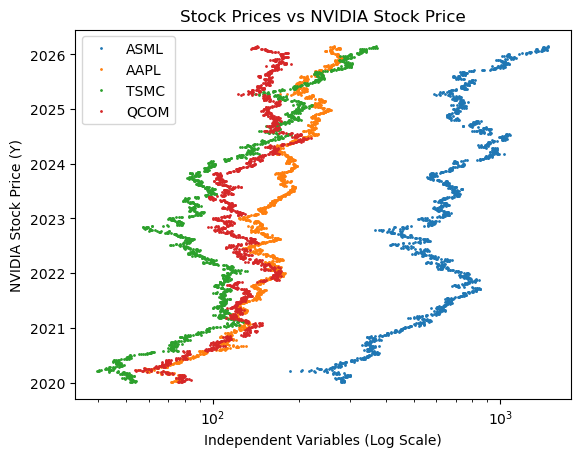
\includegraphics[width=0.9\linewidth]{group1.png}
    \caption{APA}
    \label{fig:my_image_label}
\end{figure}

\vspace{2em}

\subsection{Model 2:}

Model 2, yearly metal production, includes metals the the USGS reports on and that TSMC uses to produce NVIDIA GPUs. They have very low coefficients and thus is likely not great to predict NVIDIA's future stock price, at least not on its own. 

\begin{table}[h]
\centering
\begin{tabular}{lc}
\hline
\textbf{Metal} & \textbf{Coefficient} \\
\hline
Silver & -0.0002 \\
Tin & 2.472e-06 \\
Silicon& -1.175e-06 \\
Aluminum & 2.323e-07 \\
Rare Earths  & 2.77e-05 \\
Gold & 0.0001 \\
\hline
\end{tabular}
\caption{Regression Coefficients for Semiconductor Stocks}
\end{table}

The $R^2$ is 0.896, lower than the ideal 0.95 (for an error of 0.05 or 5\%) meaning a linear model is not the best fit for this data. However, the Breusch-Pagan and White's tests results are good. The the result of the Breusch-Pagan test, LM P-value, is 0.384 and the result of the White's test, test statistic P-value, is 0.395; these are interpreted as meaning the heteroskedasticity hypothesis is null. On the other hand, the VIFs are quite high. 

\begin{table}[h]
\centering
\begin{tabular}{lc}
\hline
\textbf{Metal} & \textbf{VIF} \\
\hline
Silver & 18.100771 \\
Tin & 1.823068 \\
Silicon& 30.965129 \\
Aluminum & 73.379265 \\
Rare Earths  & 3.287107 \\
Gold & 11.975217 \\
\hline
\end{tabular}
\caption{VIFs for yearly metal production}
\end{table}

\begin{figure}[H]
    \centering
    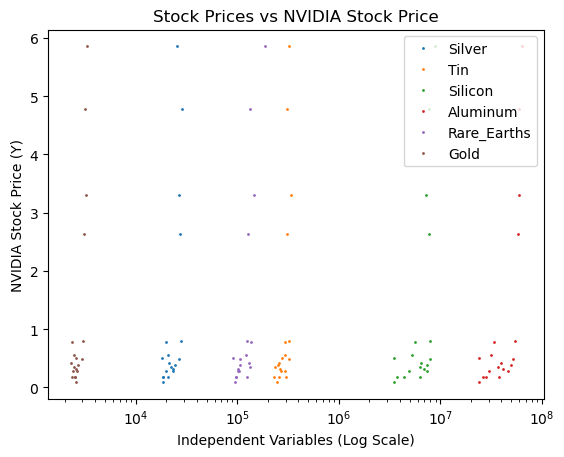
\includegraphics[width=0.9\linewidth]{group2.png}
    \caption{APA}
    \label{fig:my_image_label}
\end{figure}

In Fig 5, it is evident that most of the data is separated into unique vertical groups 

\begin{figure}[H]
    \centering
    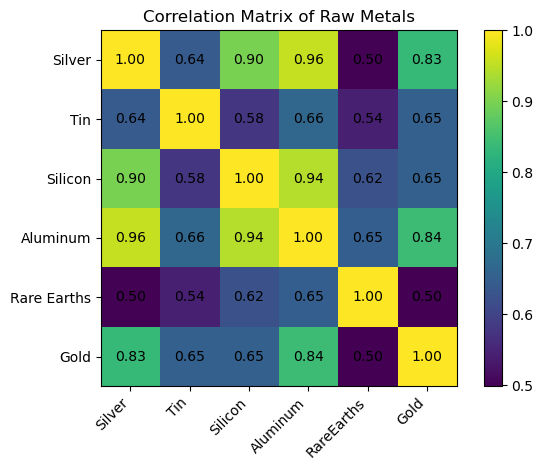
\includegraphics[width=0.9\linewidth]{group2-1.png}
    \caption{APA}
    \label{fig:my_image_label}
\end{figure}

These high VIFs could be caused by high correlation coefficients. In Fig 7 it is possible to see that the correlation coefficient between aluminum and silicon, and aluminum and silver, are quite high at 0.95; followed by aluminum and gold at 0.86. This possibly explains why aluminum has the highest VIF, as seen in table 4, at 73.38 and why gold, silver, and silicon are also high at 11.98, 12.1, and 30.97 respectively.

\subsection{Model 3:}

Model 3 consists of the daily metal futures prices for copper, gold, silver, uranium, and platinum. Chosen for their availability and relevance in GPU production or electricity production in the case of uranium. A futures contract is an agreement to buy something, in this case a metal, at a set price on a set date. For example, if a buyer agrees to buy 1 tonne of copper a week in the future for 13,000 USD, the buyer can either have a gain if the price goes over 13,000 USD at the agreed buy date or have a loss if the price goes under 13,000 USD at the agreed buy date. A bet on profit (gain) is called a speculation and when a company buys a futures contract to lock in the price it is called hedging. TSMC, for example, NVIDIA's chip supplier, could buy a futures contract for copper, gold, silicone, etc to lock in prices in the future. 

\begin{table}[h]
\centering
\begin{tabular}{lc}
\hline
\textbf{Metal Futures} & \textbf{Coefficient} \\
\hline
Copper & 12.4583 \\
Gold & 0.0934 \\
Silver  & -0.5248 \\
Platinum & -0.0711 \\
\hline
\end{tabular}
\caption{Regression Coefficients for Metals Futures}
\end{table}

\newpage

In this case the model is comparing daily close price. So, for example, if uranium changes by \$1 NVIDIA changes by \$2.4981. The model has an $R^2$ of 0.900, which is slightly lower than the ideal of 0.95. Furthermore, the Breusch-Pagan (LM = 500.44, p $<$ 0.001) and White's test ($\chi^2$ = 679.52, p $<$0.001) reject the null hypothesis of homoskedasticity. Robust standard errors (HC3) were used to account for heteroskedasticity. 

\begin{table}[h]
\centering
\begin{tabular}{lc}
\hline
\textbf{Metal Futures} & \textbf{VIF} \\
\hline
Copper & 2.063572 \\
Gold & 6.616278 \\
Silver  & 16.955074 \\
Platinum & 7.975621 \\
\hline
\end{tabular}
\caption{Regression Coefficients for Metals Futures}
\end{table}

\begin{figure}[H]
    \centering
    \includegraphics[width=0.9\linewidth]{group3-2.png}
    \caption{APA}
    \label{fig:my_image_label}
\end{figure}

The high VIFs, particularly silver's, could be explained by several factors. First, silver, gold, and platinum are all part of the precious metals industry and thus tend to move together. Secondly, in Fig 8, silver has the highest correlation coefficients at 0.92 with platinum and 0.91 with gold. Then, copper's low VIF, could be explained by first, it has the lowest correlation coefficients in Fig 8, but also, it is not part of the precious metals market meaning that it appeals to other buyers and thus doesn't move with it, making it unique in this group. 

\subsection{Model 4:}

Model 4 consists of metal ETFs. ETF means Exchange-Traded Fund. It is a type of investment fund that holds a collection of assets. GLD, SLV, and PPLT hold gold, silver, and platinum ingots, respectively; CPER holds copper futures contracts; and URA holds stocks of uranium mining companies. 

\begin{table}[h]
\centering
\begin{tabular}{lc}
\hline
\textbf{Metal ETFs} & \textbf{Coefficient} \\
\hline
Gold & 0.7454 \\
Silver & -0.1353 \\
Copper  & 0.3280 \\
Platinum & -0.9051 \\
Uranium & 2.4409 \\
\hline
\end{tabular}
\caption{Regression Coefficients for Metal ETFs}
\end{table}

These coefficients have an adjusted $R^2$ value of 0.929. This means that about 92.9\% of NVIDIA's stock movements can be explained by these metal ETFs. The metal with the biggest effect on NVIDIA's stock is Uranium. Likely because it is quickly becoming crucial for IAs. AIs need very high amounts of energy to operate and the current electric grids are struggling to meet those demands; because of this, many companies are developing modular nuclear reactors to power these IA super computers; and some of those reactors need uranium to run. The other metals are used in the production of GPUs, NVIDIA's main product. Both the Breusch-Pagan (LM = 291.99, p $<$ 0.001) and White's test ($\chi^2$ = 528.84, p $<$0.001) reject the null hypothesis of homoskedasticity. Robust standard errors (HC3) were used to account for heteroskedasticity. 

\begin{table}[h]
\centering
\begin{tabular}{lc}
\hline
\textbf{Metal ETFs} & \textbf{VIFS} \\
\hline
Gold & 9.303403 \\
Silver & 17.051093 \\
Copper  & 3.061417 \\
Platinum & 7.710108 \\
Uranium & 6.072512 \\
\hline
\end{tabular}
\caption{Regression Coefficients for Metal ETFs}
\end{table}

\begin{figure}[H]
    \centering
    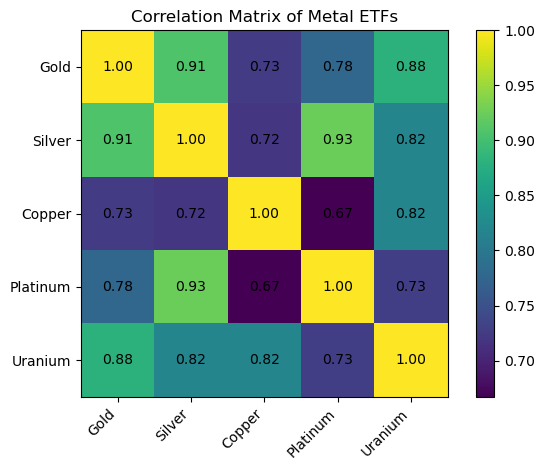
\includegraphics[width=0.9\linewidth]{group4-1.png}
    \caption{APA}
    \label{fig:my_image_label}
\end{figure}

The high VIFs, seen in Table 8, for gold, silver, and platinum, as in group 3, can be attributed to them being in the same industry and them having the highest correlation coefficients between them. Then, uranium's high VIF at 6, could possibly be explained by its correlation coefficients mostly staying in the 0.8-0.9 range except for platinum which is lower at 0.7. And lastly, as seen in group 3 as well, copper is in a sepparate industry to all the other metals plus it has the lowest overall correlation coefficients. 

\subsection{Model 5:}

The S\&P 500 is a stock index that tracks the 500 largest US companies, weighted by market cap. It is widely considered the best single measure of large-cap US companies and an overall measure of market health. Compared to other indexes, it also serves as the best measure of overall US economic health. This can be compared to the NVIDIA stock although currently NVIDIA is part of the 500 companies. For this model I am using the daily percentage change for both stocks. 

\begin{table}[h]
\centering
\begin{tabular}{lc}
\hline
\textbf{Index} & \textbf{Coefficient} \\
\hline
S\&P 500 & 1.7839 \\
\hline
\end{tabular}
\caption{Regression Coefficient for S\&P 500}
\end{table}

The coefficient of 1.7839 means that for every 1\% the S\&P 500 moves, NVIDIA will move 1.7839\% in the same direction (+ or -). The $R^2$ of 0.493 means that about 49\% of NVIDIA's stock movements can be explained by the S\&P 500's movements. Which for a single stock is quite high. A Breusch-Pagan test revealed significant heteroskedasticity in the model (LM = 135.43, p $<$ 0.001) and a White's test revealed even stronger evidence($\chi^2$ = 384.81, p $<$ 0.001), this means the model rejects the null hypothesis of homoskedasticity. Robust standard errors (HC3) were used to account for heteroskedasticity. Furthermore, the VIF test returned a value of 1, although this is expected since only one stock is being compared to NVIDIA. Overall, the S\&P 500 is a good variable to use in a linear regression model comparing \%$\Delta$  of both stocks to predict the future \%$\Delta$ of NVIDIA's daily close price. 

\begin{figure}[H]
    \centering
    \includegraphics[width=0.9\linewidth]{group5.png}
    \caption{APA}
    \label{fig:my_image_label}
\end{figure}

\subsection{Model 6:}

The NASDAQ 100 index represents all stocks and companies traded on the NASDAQ exchange. It works similar to the S\&P 500, each company has a weight assigned to it based on its market value. For example, NVIDIA's weight is currently (3/2/2026) 12.96\%. But in difference to the S\&P 500, the NASDAQ mostly centers around tech companies, making it more suitable for predicting NVIDIA's daily close price since NVIDIA is a major component of the index and shares similar market drivers with other tech stocks in the index. Furthermore, the adjusted $R^2$ returned a value of 0.649, meaning that 65\% of NVIDIA's changes can be explained by NDX. 

\begin{table}[h]
\centering
\begin{tabular}{lc}
\hline
\textbf{Index} & \textbf{Coefficient} \\
\hline
NDX & 1.6695 \\
\hline
\end{tabular}
\caption{Regression Coefficient for NASDAQ 100}
\end{table}



The coefficient of 1.6695 means that for every 1\% change in NDX, NVDA changes by 1.6695\% in the same direction (+ or -). Furthermore, the Breusch-Pagan (LM = 75.50, p $<$ 0.001) and White's test ($\chi^2$ = 132.93, p $<$ 0.001) both strongly reject the null hypothesis of homoskedasticity. Robust standard errors (HC3) were used to account for heteroskedasticity. Moreover, the VIF test returned a value of 1, which is expected since only one variable is being compared to NVIDIA. Overall, the NDX index is a good variable for predicting the daily \%$\Delta$ of NVIDIA's daily close price using a linear regression model comparing the daily \%$\Delta$ of both stocks. 

\begin{figure}[H]
    \centering
    \includegraphics[width=0.9\linewidth]{group6-1.png}
    \caption{APA}
    \label{fig:my_image_label}
\end{figure}

\subsection{Model 7:}

AI data centers need high amounts of electricity, but current electric grids are struggling to meet the demand. Because of this, many AI companies, like Google, Meta, OpenIA, etc, are investing in modular nuclear reactors to power their data centers. There are many companies that make these, for example Oklo. Oklo is an American company founded in 2013 that focuses on developing small modular reactors (SMRs up to 300 MW). Another example is Nano nuclear, a company that develops micro modular reactors (MMR typically under 10-20 MW). These reactors would be placed next to or near data centers to power them while at the same time also isolating them from the greater grid which can be vulnerable to outages which can cost AI companies billions of dollars. 

\begin{table}[h]
\centering
\begin{tabular}{lc}
\hline
\textbf{SMR and MMR Company Stocks} & \textbf{Coefficients} \\
\hline
NuScale & 0.3682 \\
Oklo & -0.0811 \\
GE Vernova   & 0.0176 \\
BWX & 0.6739 \\
Nano Nuclear  & 0.0078 \\
\hline
\end{tabular}
\caption{Coefficients for SMR and MMR Company Stocks}
\end{table}

These coefficients, along with an $R^2$ of 0.906 shows a decent relationship between these stocks and NVIDIA's stock. Furthermore, both the Breusch-Pagan (LM = 49.07, p $<$ 0.001) and White's test ($\chi^2$ = 138.58, p $<$ 0.001) strongly reject the null hypothesis of homoskedasticity. Robust standard errors (HC3) were used to account for heteroskedasticity. 

\begin{table}[h]
\centering
\begin{tabular}{lc}
\hline
\textbf{SMR and MMR Company Stocks} & \textbf{VIFS} \\
\hline
NuScale & 3.252240 \\
Oklo & 9.275726 \\
GE Vernova   & 7.662576 \\
BWX & 10.590868 \\
Nano Nuclear  & 5.090562 \\
\hline
\end{tabular}
\caption{VIFs for SMR and MMR Company Stocks}
\end{table}

\begin{figure}[H]
    \centering
    \includegraphics[width=0.9\linewidth]{group7-1.png}
    \caption{APA}
    \label{fig:my_image_label}
\end{figure}

The high VIFs for these stocks like stem from the fact that they are all in the same niche industry. Furthermore, they all respond to the same nuclear policy news, uranium prices, and energy sector trends. NuScale's low VIF could be explained by the fact that they are the most developed of the companies, being the only ones to have gotten Nuclear Regulatory Commission approval. Furthermore, BWX has the highest VIF and correlation coefficients; while NuScale has the lowest. 

\section{Conclusion}

Overall, all the models demonstrate a significant ability to predict NVIDIA's stock movements. But they do have a strong limitation, the change in the predictor stock has to happen before the change in NVIDIA but the models all have changes in the same date for both the predictor and NVIDIA. Nevertheless, the results are promising. Overall, the models can be divided into 4 tiers, first tier (best) are model 1 and model 4 with the hightest $R^2$ at 0.97 and 0.93 respectively, although model 1 does have high VIFs; second tier (good predictors) are models 7 and 3, their $R^2$ are good but not great at 0.906 and 0.900 respectively, furthermore Uranium's coefficient in model 4 is the highest at 2.44; third tier (moderate predictors) are model 6 and 5 with $R^2$ of 0.649 and 0.493 respectively, the $R^2$ are low but considered moderate since they represent one single parameter, these models are good but not on their own, they need to be combined with other parameters to be more effective; and lastly fourth tier (weakest) model 2 with an $R^2$of 0.896 and extreme VIFs. To answer the question, what parameters are best to predict the stock close price of NVIDIA when using a linear regression model to make the prediction? and using the data from the models above, I have created what I call Model Ultimate. 

\subsection{Model Ultimate}

Model Ultimate consists of a mix of parameters from models 1, 4 and 6. 

\begin{table}[h]
\centering
\begin{tabular}{lc}
\hline
\textbf{Parameter} & \textbf{Coefficient} \\
\hline
ASML & -0.0803 \\
Uranium ETF   & 1.2540 \\
Nasdaq 100 & 0.0131 \\
\hline
\end{tabular}
\caption{Model Ultimate Coefficients with Newey-West Standard Errors}
\end{table}

These 3 parameters where found to be the best due to their acceptable VIFs, high $R^2$ (0.932), and perfect Breusch-Pagan and White's test results. The uranium ETF's coefficient (1.254) dominates, reflecting AI's energy demands, while NASDAQ captures tech sector sentiment and ASML shows negative correlation possibly from portfolio rebalancing. The Breusch-Pagan (LM = 187.45, p $<$ 0.001) and White's test ($\chi^2$ = 609.77, p $<$ 0.001) strongly reject the null hypothesis of homoskedasticity. Newey-West (HAC) standard errors with 8 lags were applied to account for both heteroskedasticity and autocorrelation. All coefficients remain highly significant (p < 0.001). The Durbin-Watson statistic of 0.024 indicates severe autocorrelation, common in financial time series. While Newey-West standard errors correct for this in our hypothesis tests, time series models would be better for out-of-sample forecasting.

\begin{table}[h]
\centering
\begin{tabular}{lc}
\hline
\textbf{Parameter} & \textbf{VIF} \\
\hline
ASML & 4.179405 \\
Uranium ETF   & 7.562880 \\
Nasdaq 100 & 7.107493 \\
\hline
\end{tabular}
\caption{VIFs for Model Ultimate}
\end{table}

The VIFs are acceptable. Ideally, they would be lower (closer to 1), but for the scope of this essay they will do. 

\begin{figure}[H]
    \centering
    \includegraphics[width=0.9\linewidth]{groupU-1.png}
    \caption{APA}
    \label{fig:my_image_label}
\end{figure}

The high VIFs for the uranium ETF and Nasdaq 100 could be due to the high correlation coefficient at 0.92, but it could also be attributed to the fact that most, if not all, of the companies in the nasdaq 100 (tech companies) depend on the energy sector to exist. 
\\ \\
These parameters best explain NVIDIA's historical price movements (R² = 0.932), with uranium's dominance highlighting how NVIDIA's valuation has evolved into a broader bet on AI infrastructure rather than traditional semiconductor fundamentals.
\\ \\
Key limitations include: simultaneous rather than lagged predictor changes, severe autocorrelation suggesting time series models would be superior, correlation not causation, and NASDAQ circularity (NVIDIA is 13\% of the index). Historical relationships may not persist if AI market dynamics shift.

\newpage

\section{Bibliography}

\begin{itemize}
    \item R1B0PR07008. (2026). \textit{Clean Data Fixed from Model 7.ipynb} (Version from School-Public repository) [Jupyter Notebook]. GitHub. \url{https://github.com/R1B0PR07008/School-Public/blob/main/Extended%20Essay/Clean%20Data%20Fixed%20from%20Model%207.ipynb}
    \item Yahoo Finance. (n.d.). \textit{Yahoo Finance}. Yahoo. \url{https://finance.yahoo.com/}
    \item Oklo Inc. (n.d.). \textit{About Oklo}. Oklo. \url{https://oklo.com/about/default.aspx}
    \item Reuters. (2025, August 5). \textit{Intel struggles with key manufacturing process for next PC chip, sources say}. Reuters. \url{https://www.reuters.com/world/asia-pacific/intel-struggles-with-key-manufacturing-process-next-pc-chip-sources-say-2025-08-05/}
    \item U.S. Geological Survey. (n.d.). \textit{Platinum-group metals statistics and information}. U.S. Department of the Interior. \url{https://www.usgs.gov/centers/national-minerals-information-center/platinum-group-metals-statistics-and-information}
    \item U.S. Geological Survey. (n.d.). \textit{Silver statistics and information}. U.S. Department of the Interior. \url{https://www.usgs.gov/centers/national-minerals-information-center/silver-statistics-and-information}
    \item U.S. Geological Survey. (n.d.). \textit{Rare earths statistics and information}. U.S. Department of the Interior. \url{https://www.usgs.gov/centers/national-minerals-information-center/rare-earths-statistics-and-information}
    \item U.S. Geological Survey. (n.d.). \textit{Gold statistics and information}. U.S. Department of the Interior. \url{https://www.usgs.gov/centers/national-minerals-information-center/gold-statistics-and-information}
    \item U.S. Geological Survey. (n.d.). \textit{Aluminum statistics and information}. U.S. Department of the Interior. \url{https://www.usgs.gov/centers/national-minerals-information-center/aluminum-statistics-and-information}
    \item U.S. Geological Survey. (n.d.). \textit{Silicon statistics and information}. U.S. Department of the Interior. \url{https://www.usgs.gov/centers/national-minerals-information-center/silicon-statistics-and-information}
    \item U.S. Geological Survey. (n.d.). \textit{Copper statistics and information}. U.S. Department of the Interior. \url{https://www.usgs.gov/centers/national-minerals-information-center/copper-statistics-and-information}
    \item Gujarati, D. N. (2011). \textit{Econometrics by example}. Palgrave Macmillan.
    \item Malhotra, N., \& Tandon, K. (2013). \textit{Determinants of stock prices: Empirical evidence from NSE 100 companies}. \textit{International Journal of Research in Management \& Technology, 3}(3), 86--90.
\end{itemize}

\end{document}